\documentclass{article}
\usepackage[utf8]{inputenc}
\usepackage{amsmath,amssymb,amsfonts}
\usepackage{amsthm}
\let\oldAA\AA
\renewcommand{\AA}{\text{\normalfont\oldAA}}
\usepackage[makeroom]{cancel}
\usepackage{graphicx}
\usepackage{subcaption}
\usepackage{caption}{\tiny }
\usepackage[affil-it]{authblk}
\usepackage{multirow}
\usepackage[table,xcdraw]{xcolor}
\usepackage{titlesec}
\usepackage{longtable}
\usepackage{wrapfig}
\usepackage{mathtools}
\usepackage{braket}
\usepackage{bm}
\usepackage{esvect}
\usepackage[colorlinks = true,
            linkcolor =  black,
            urlcolor  = blue,
            citecolor = blue,
            anchorcolor = blue]{hyperref}

\newcommand{\MYhref}[3][blue]{\href{#2}{\color{#1}{#3}}}%
\usepackage[
bookmarksopen,
bookmarksdepth=2,
breaklinks=true
]{hyperref}
\usepackage{arxiv}
\usepackage[utf8]{inputenc} % allow utf-8 input
\usepackage[T1]{fontenc}    % use 8-bit T1 fonts
\usepackage{hyperref}       % hyperlinks
\usepackage{url}            % simple URL typesetting
\usepackage{booktabs}       % professional-quality tables
\usepackage{amsfonts}       % blackboard math symbols
\usepackage{nicefrac}       % compact symbols for 1/2, etc.
\usepackage{microtype}      % microtypography
\usepackage{lipsum}		% Can be removed after putting your text content
\usepackage{graphicx}
\usepackage{natbib}
\usepackage{doi}
\renewcommand\refname{}
\renewcommand*\contentsname{}



\title{NSLS-II}

\date{17 Ocak 2022}


\author{ \href{https://orcid.org/0000-0002-1684-9602}{
\includegraphics[scale=0.06]{orcid.pdf}\hspace{1mm}Halil Kolatan} \\
	Ankara Üniversitesi\\
	Fen Fakültesi 
	Fizik Bölümü }\\
	%halilkolatan@gmail.com	}
% Uncomment to remove the date

% Uncomment to override  the `A preprint' in the header
%\renewcommand{\headeright}{Technical Report}
%\renewcommand{\undertitle}{Technical Report}
%\renewcommand{\shorttitle}{\textit{arXiv} Template}

%%% Add PDF metadata to help others organize their library
%%% Once the PDF is generated, you can check the metadata with
%%% $ pdfinfo template.pdf
\hypersetup{
pdftitle={NSLS-II},
pdfsubject={NSLS-II Proje Ödevi},
pdfauthor={Halil }
pdfkeywords={Plazma},
}

\begin{document}
\maketitle
\begin{abstract}
\tableofcontents
\end{abstract}
\section{Giriş}
 Parçacık fiziğinde keşif arayışı her zaman mümkün olan en yüksek enerjilerde deneyler gerektirmiştir. Yüksek enerjili parçacık hızlandırıcılar ise şimdiye kadar parçacık fiziğinin doğasını anlamak için vazgeçilmez bir araç olmuştur. Parçacık demetlerini çok yüksek enerjiyle hızlandırmak, bu demetleri çarpıştırmak ve bu çarpışmaların oluşturduğu parçacıkları tespit etmek için yeni teknikler geliştirilmiştir. Standart Modelin (SM) ötesinde, daha yüksek bir enerji seviyesinde yeni parçacıklar arayışını sürdürebilecek bir tesis yaratmak için teknikte daha fazla ilerleme gereklidir. Bu ilerlemenin sonucunda artık hızlandırıcılar ve ışınım kaynakları birçok alanda kullanılmaktadır. Günümüzde ülkeler, birçok ışınım ve hızlandırıcı kompleksi kurarak bu ilerlemelere öncülük etmektedirler. Bu çalışmada, dünyanın en gelişmiş ışınım kaynaklarından biri olan Brookhaven Ulusal Laboratuvarı'ndaki Ulusal Sinkrotron Işınım Kaynağı  II (NSLS-II) incelenecektir.
  \newpage
  
\section{NSLS II}

	\begin{figure}[h!]
 \centering

\includegraphics[width=13cm]{ssözet.png}
\caption*{Şekil 1. NSLS-II Tesisi [1].}
	\end{figure}

New York, Upton'daki Brookhaven Ulusal Laboratuvarı'ndaki (BNL) Ulusal Sinkrotron Işınım Kaynağı II (NSLS-II), öncelikle ABD Enerji Bakanlığı'nın (DOE) Bilim Ofisi tarafından finanse edilen bir ulusal kullanıcı araştırma tesisidir. NSLS-II, BNL'nin orijinal ışınım kaynağı olan Ulusal Sinkrotron Işınım Kaynağından (NSLS) 10.000 kat daha parlak x-ışınları üretmek üzere tasarlanmış, dünyanın en gelişmiş sinkrotron ışınım kaynaklarından biridir [2].

Yoğun ultra parlak ışığını yaratmak için NSLS-II, elektronları yarım mil (791.958 m) uzunluğundaki halkasının etrafında neredeyse ışık hızında döndüren gelişmiş bir parçacık hızlandırıcı kompleksine sahiptir. NSLS-II'nin hızlandırıcıları birçok karmaşık mühendislik sisteminden oluşur. Bu yoğun, kararlı elektron demetini her yıl 5000 saat kesintisiz olarak çalıştırmak, her entegre bileşene sürekli dikkat gerektirmektedir [3].

NSLS-II'deki disiplinler arası ekipler, dünyanın dört bir yanından gelen araştırmacılarla ortak çalışarak malzemelerin atomik yapısını, temel yapısını ve elektronik davranışlarını ortaya çıkarıyor. Bu yeni, daha derin malzeme anlayışını yaratarak, bu araştırma ekipleri yaşam bilimleri, enerji depolama, ileri malzeme bilimi, fizik, kimya ve biyoloji gibi çok çeşitli bilimsel disiplinlerdeki bilgimizi geliştirmektedir [2].

Şu anda, NSLS-II'nin işletimde olan 28 demet hattı ve yapım aşamasında olan 4 ek demet hattı bulunmaktadır. Depolama halkası rutin olarak 400 mA ve 30 pm-rad dikey yayılımda ve özel çalışma periyotlarında 8 pm-rad'da çalıştırılır. NSLS-II, hızlandırıcı sistemler için çok yıllı bir geliştirme planı uygulamaktadır. Bu tamamlandığında, NSLS -II depolama halkasının 500 mA ve 8 pm -rad dikey emisyon gibi yüksek performans spesifikasyonlarında güvenilir bir şekilde çalıştırılacaktır [4].

NSLS-II, 2015 yılında kullanıcı işlemlerine başladı. 2019 yılında, 1755 farklı araştırmacı araştırmaları için NSLS-II demet hatlarını kullandı. 2020 yılında bu sayı, küresel COVID-19 pandemisinin etkisiyle 1355 oldu. Buna rağmen, NSLS-II 2020 yılında 577 yayın yaptı ve bu yayınların \%40'ından fazlası etki faktörü 7.0'dan büyük olan dergilerde yer aldı ve bu NSLS-II'nin başarısını göstermektedir [4].

\begin{figure}[h]
\centering
\begin{subfigure}{0.4\textwidth}
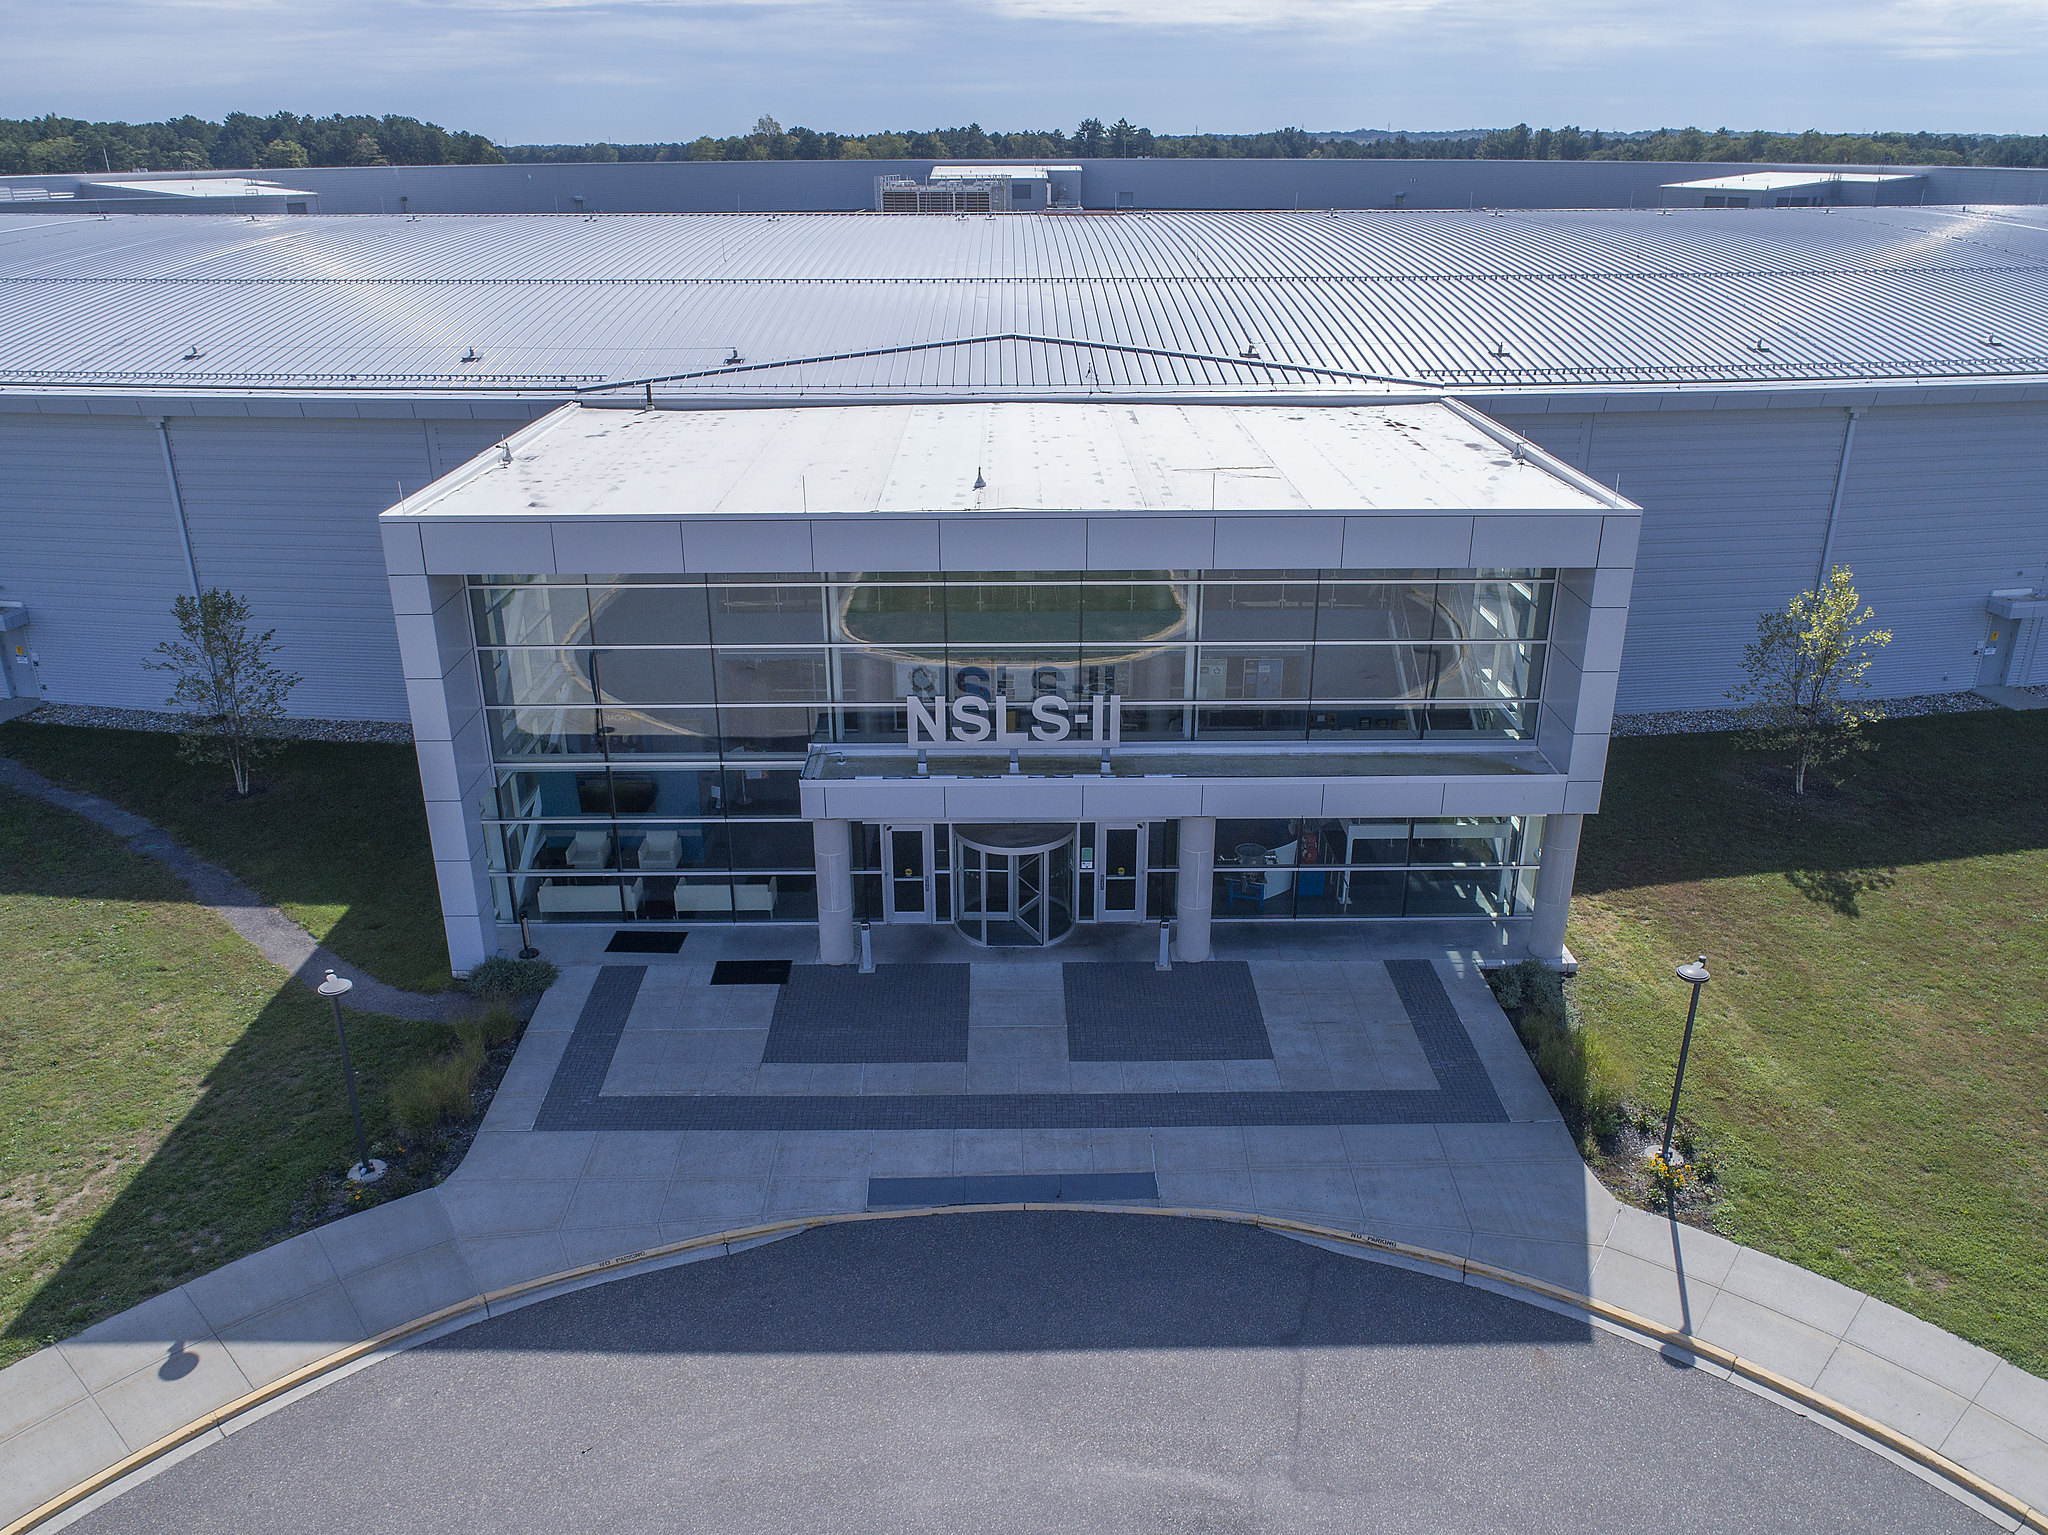
\includegraphics[width=1\linewidth]{27597220709_1e50948a52_k.jpg}
\end{subfigure}	
\begin{subfigure}{0.4\textwidth}	
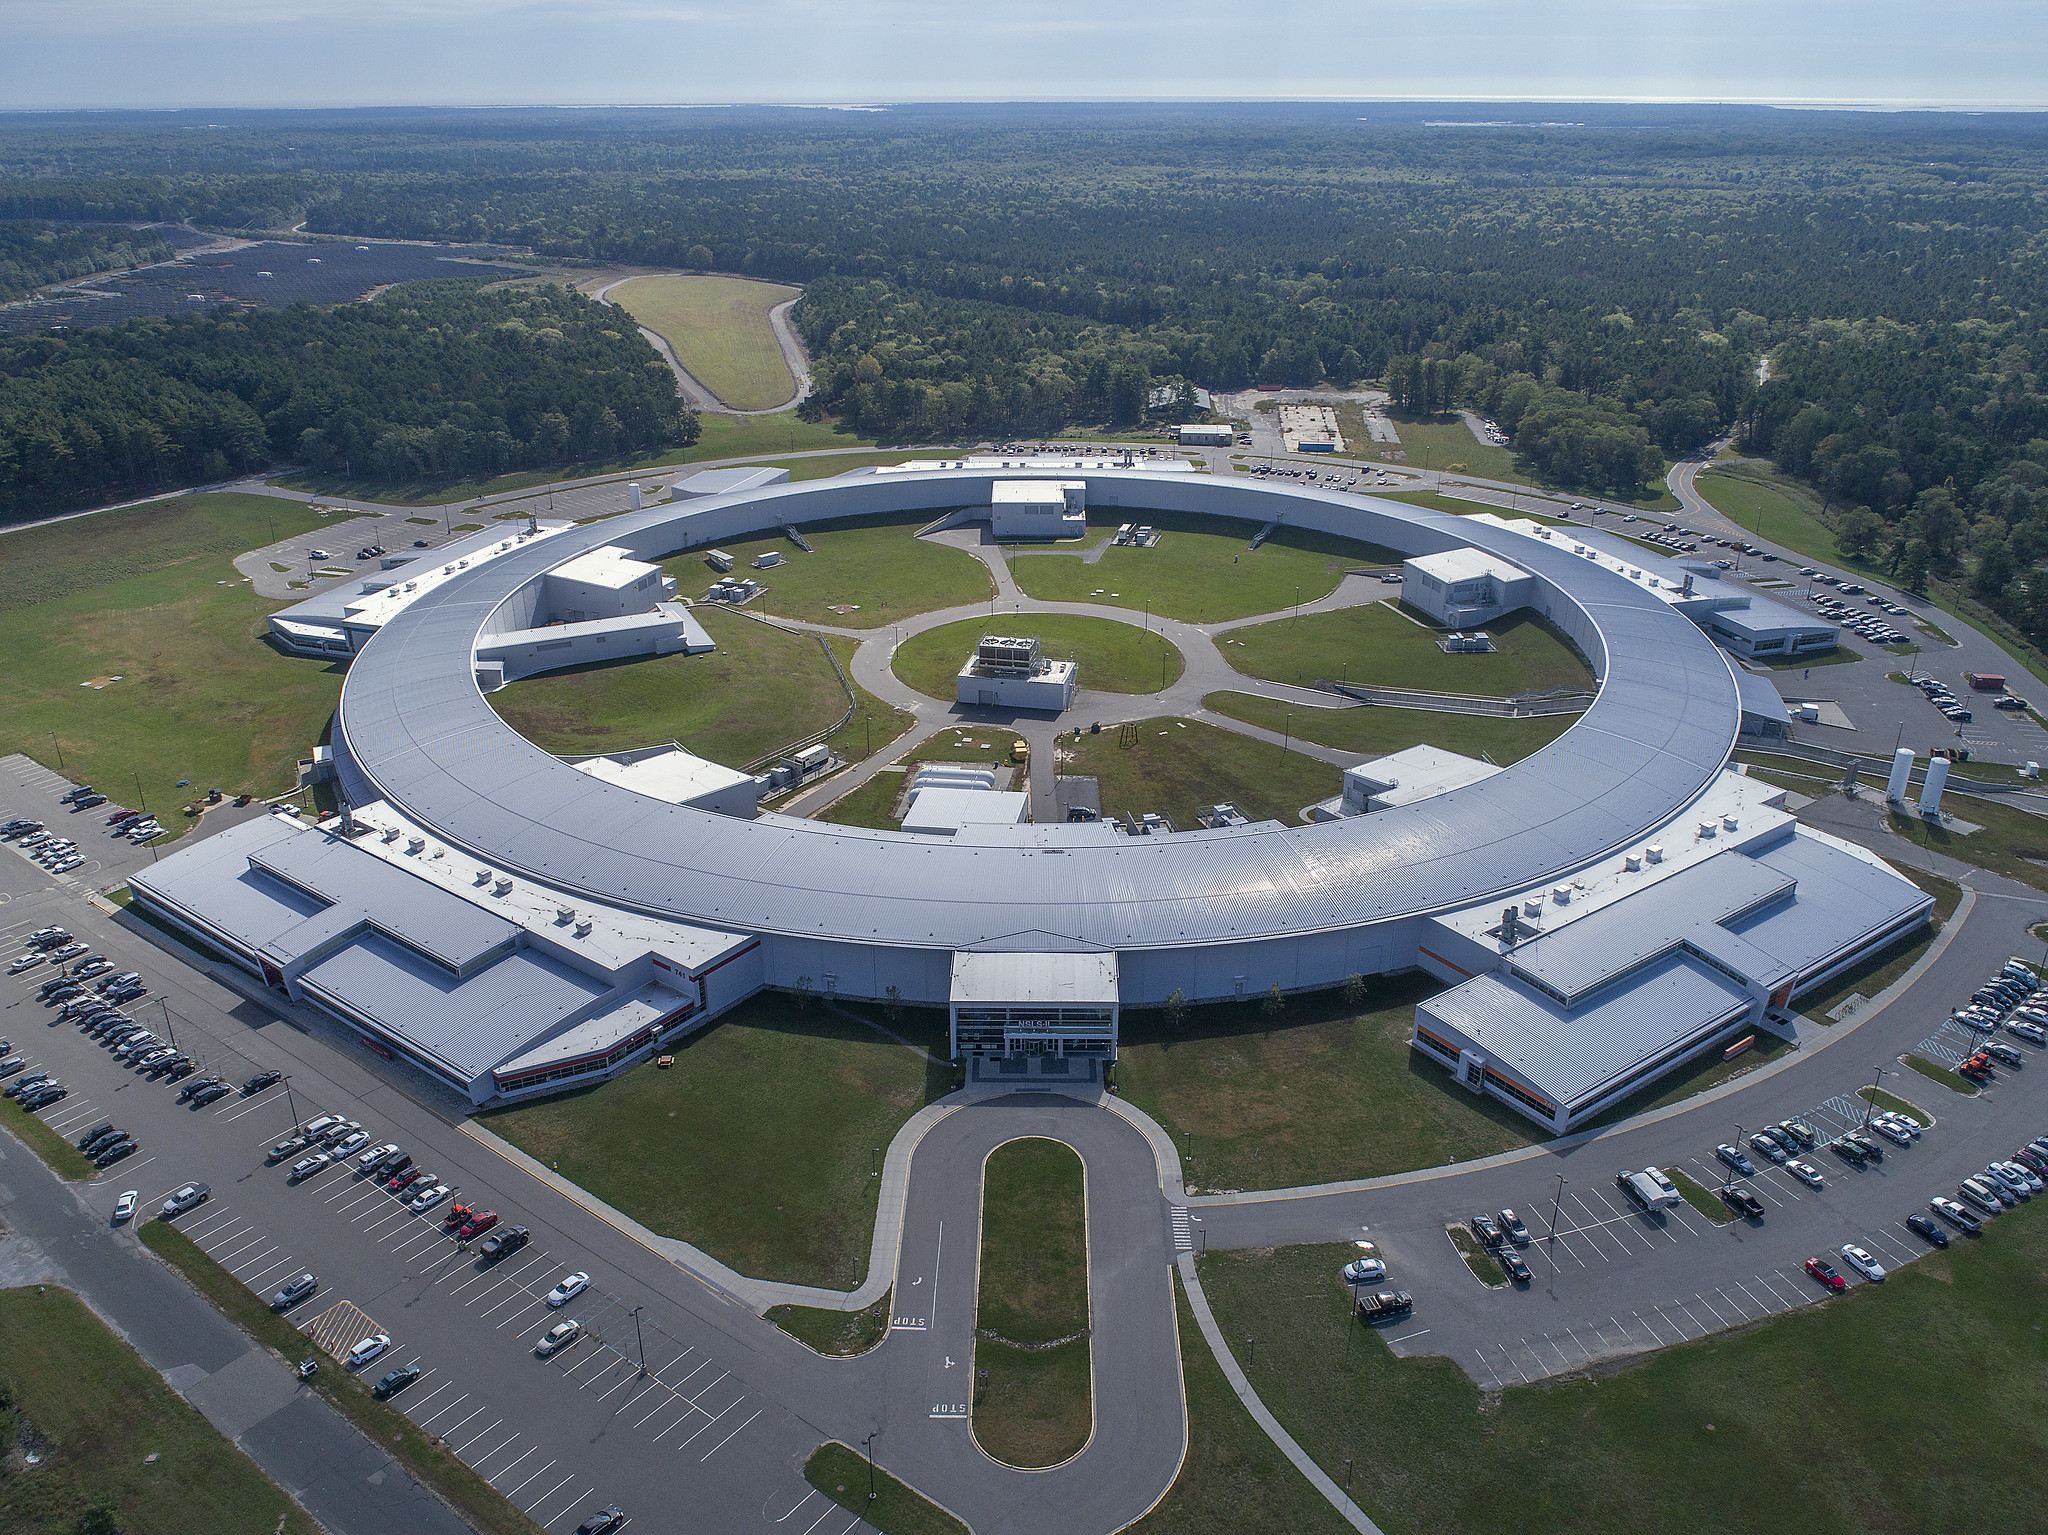
\includegraphics[width=1\linewidth]{39344406832_b5a2641959_k.jpg}
\end{subfigure}
\caption*{Şekil 2. NSLS-II Tesisi [1].}
\end{figure}
   
   
   
   \newpage
   

\section{NSLS II Tesis Tasarımı}


	
	\begin{figure}[h]
 \centering
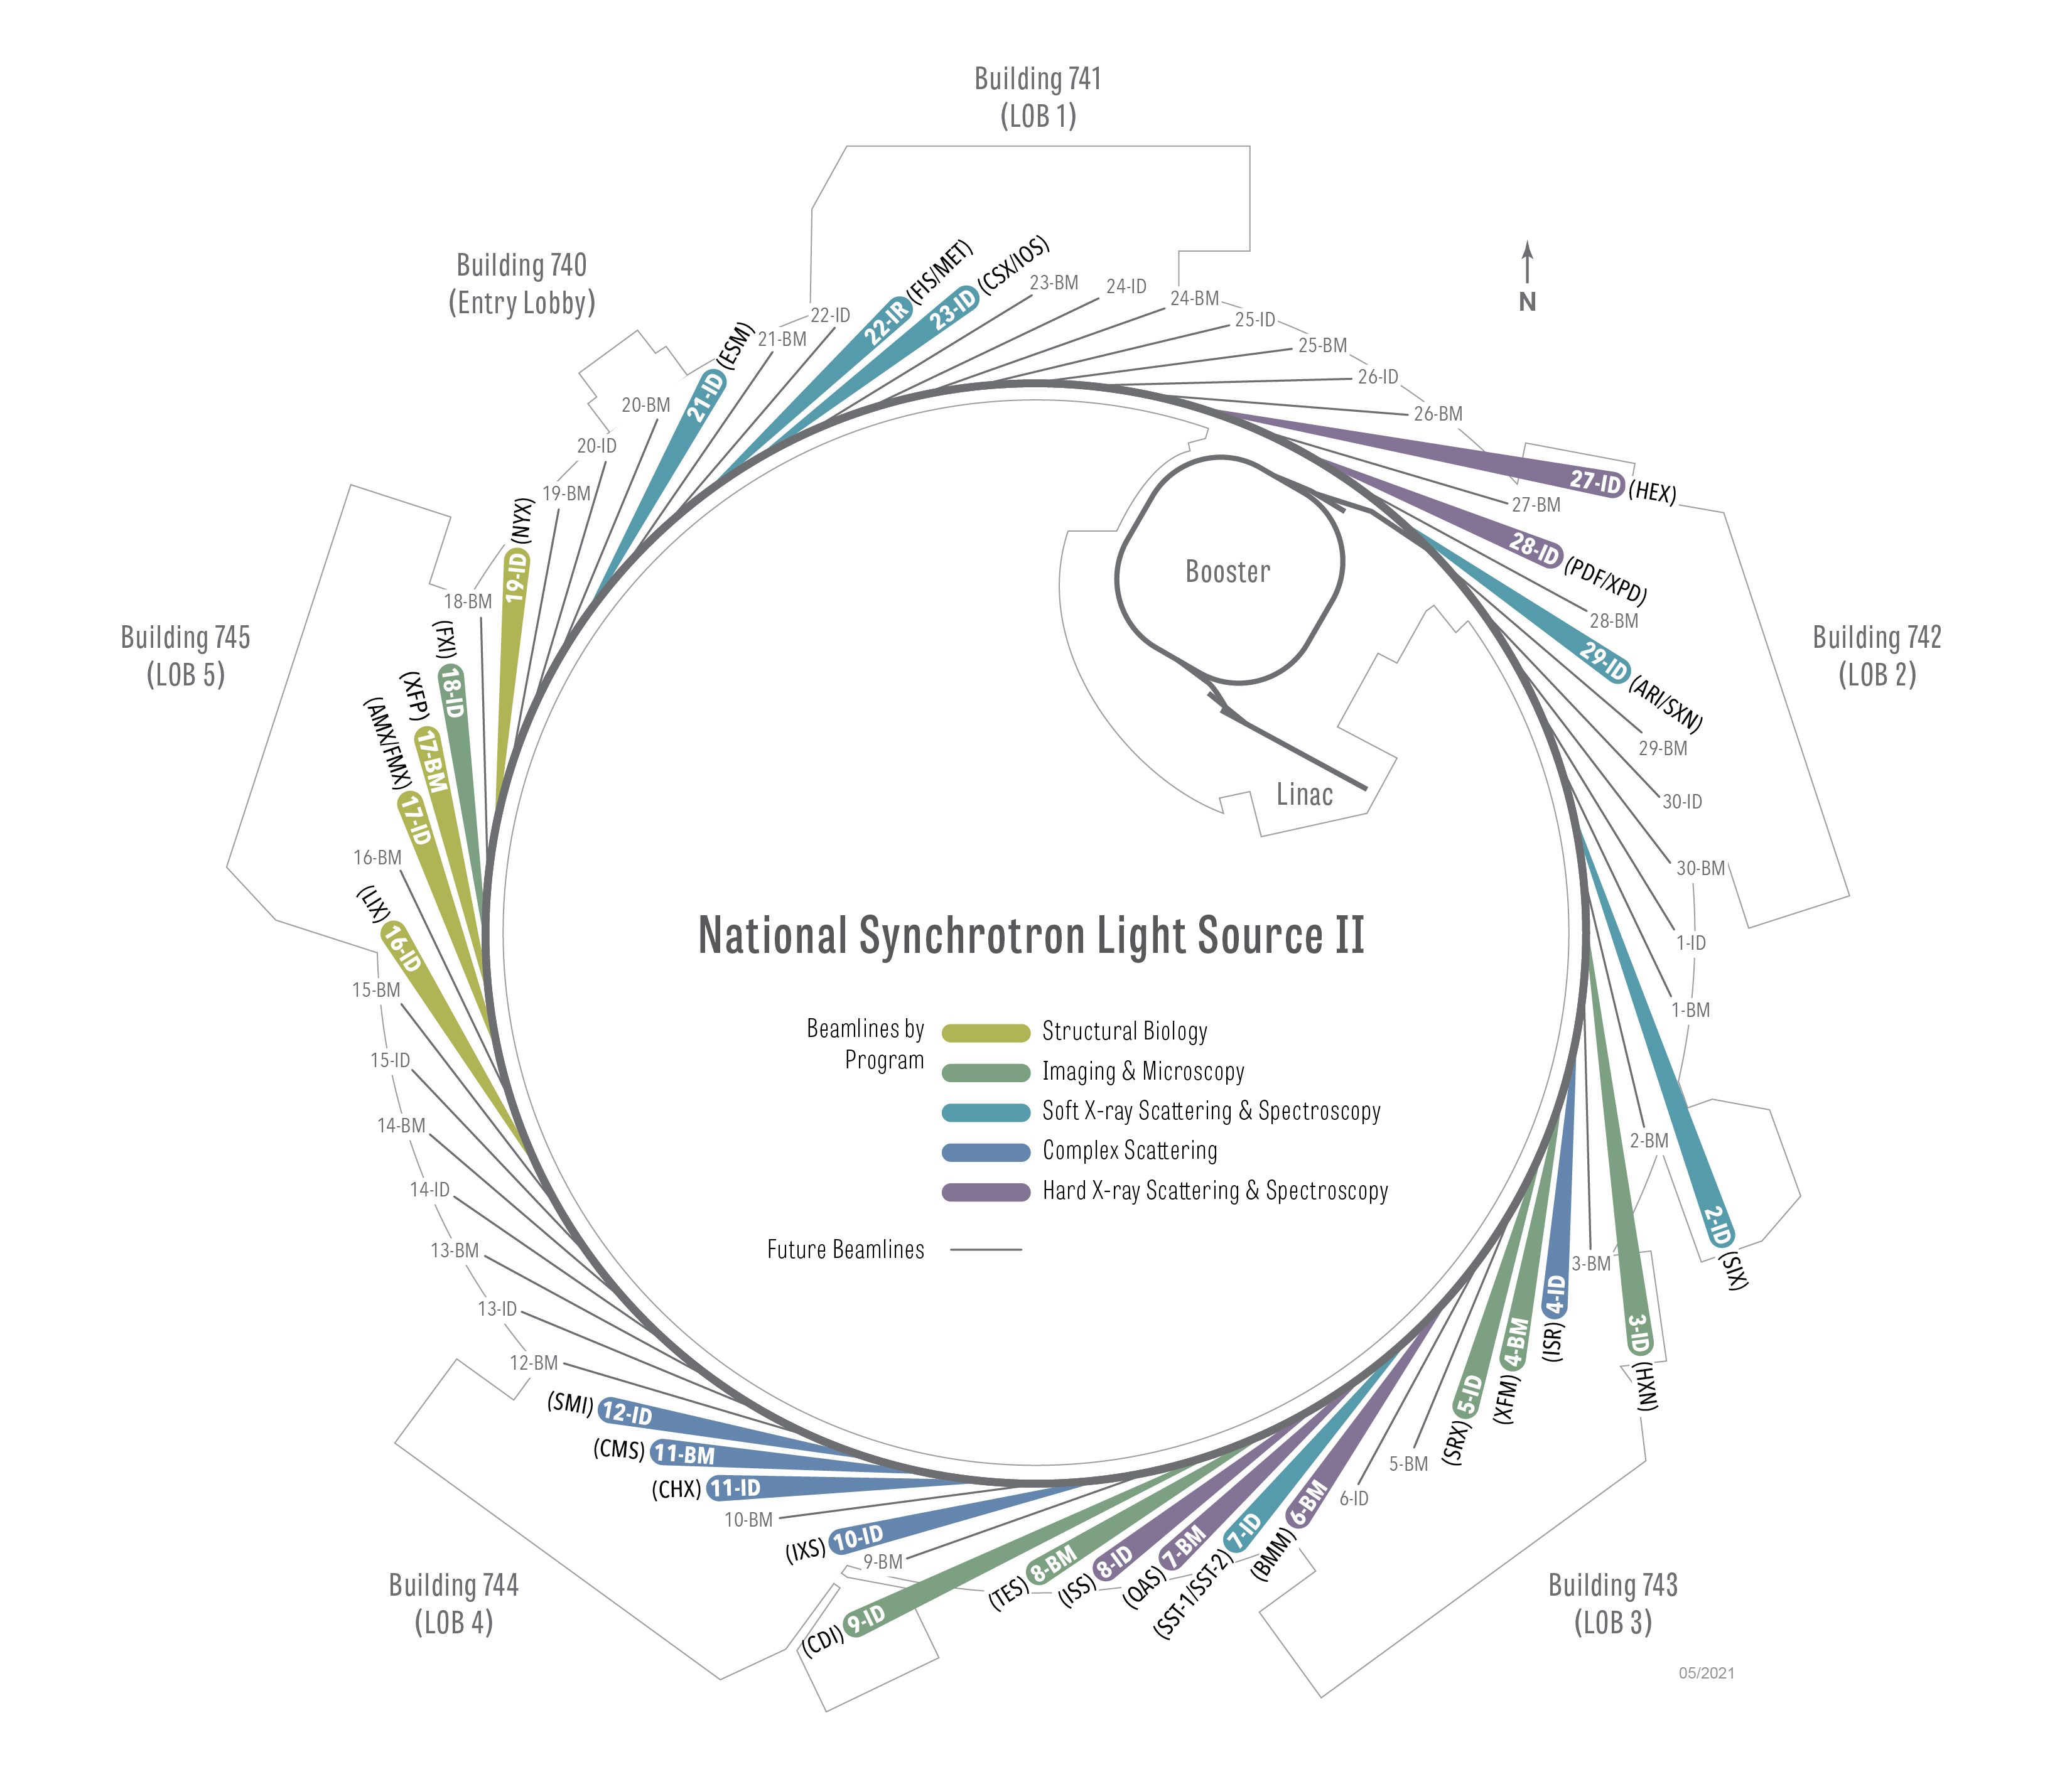
\includegraphics[width=16cm]{nsls2-beamlinesclock-jpg.jpg}
\caption*{Şekil 3. NSLS-II Demet hattı haritası [6].}
	\end{figure}
	
	Ulusal Sinkrotron Işınım Kaynağı II (NSLS-II) hızlandırıcı kompleksi, elektronların yaratılmasından parlak sinkrotron ışınımının üretilmesine kadar her şeyi kapsamaktadır. NSLS-II hızlandırıcı kompleksi bir elektron tabancası, bir lineer hızlandırıcı, bir güçlendirici halka ve depolama halkasından oluşur. İlk üç bölüm, elektronları depolama halkası boyunca yolculuklarına hazırlamak için gereklidir, orta enerjili elektron depolama halkası ise parlak ışınım demetleri üreten tüm cihazları içerir [7].
	
	Depolama halkasını barındıran deney salonu, 60 demet hattına kadar, hafif taşıma hatlarının bir kombinasyonu ve deney istasyonları için yeterli alan sunar. Bu demet hatları 66 metre ila 72 metre uzunluğunda olabilir. NSLS-II ayrıca, bitişik bir binada bulunan deney istasyonları ile mevcut binanın ötesine geçebilen dokuz ekstra uzun demet hattını barındırabilir. Bu demet hatları yaklaşık 200 m uzunluğundadır [7].
	
	\newpage
	
\subsection{Lineer Hızlandırıcı}

	\begin{figure}[h]
 \centering
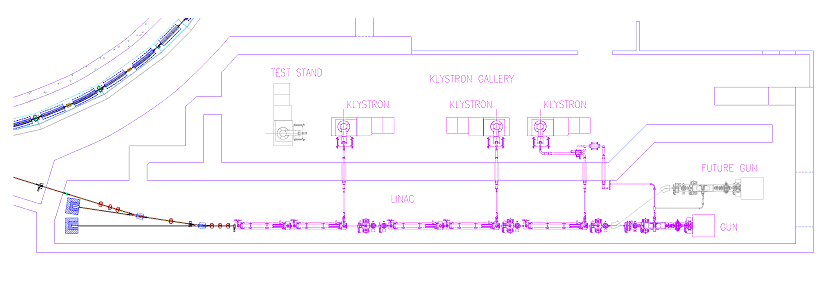
\includegraphics[width=12cm]{linacss.png}
\caption*{Şekil 4. 200 MeV lineer hızlandırıcının düzeni [8].}
	\end{figure}
	
NSLS-II lineer hızlandırıcı, BNL ile işbirliği içinde RI Research Instruments, GmbH tarafından geliştirilmiş 200 MeV normal iletken bir lineer hızlandırıcıdır. Bir DC termiyonik elektron Tabancası, demetleme sistemi ve dört adet 3 GHz TW yapısından oluşur. Tabanca tek demet ve çoklu demet modu olmak üzere iki modda çalışabilir.Demetleme bölümü, demet uzunluğunu ns'den $\sim$ 10 ps'ye sıkıştırmak için tasarlanmış 500 MHz alt harmonik ön demetleyici, 3 GHz ön demetleyici ve 3 GHz hareketli dalga demetleyiciden oluşur. Dört adet 3 GHz hareketli dalga yapısı, ışını 200 MeV'ye kadar hızlandırır. Lineer hızlandırıcıya RF gücü sağlamak için üç klistron mevcuttur; bunlardan ikisi kullanımdadır ve üçüncüsü bir klistron arızası durumunda yedektedir. Lineer hızlandırıcıdan, güçlendirici halkaya transfer hattında biri lineer hızlandırıcının kendisinden sonra diğeri de enerji spektrometresinden sonra olmak üzere iki demet kapanı vardır [9].


\subsection{Güçlendirici Halka}

			\begin{figure}[h]
 \centering
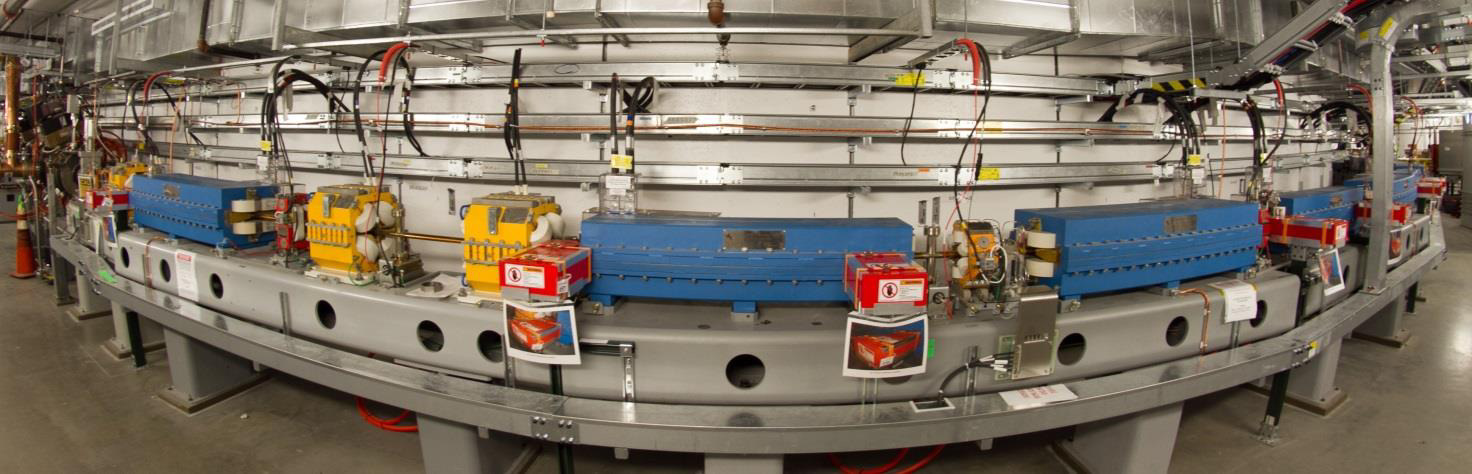
\includegraphics[width=12cm]{booster.png}
\caption*{Şekil 5. NSLS-II Güçlendirici halka [10].}
	\end{figure}
	
Güçlendirici halkanın çevresi 158,4 metredir ve 60 odaklayıcı dipollü dört dönem birleşik işlevli FODO örgüsü içerir. Güçlendirici manyetik alan ve RF voltajı, demeti 200 MeV'den 3 GeV'a hızlandırmak için yükseltilir. Maksimum dipol alanı 1 T'dır. RF gücü, 90 kW IOT tabanlı bir verici sistemi tarafından sürülen PETRA 7 hücreli 500 MHz Cu-kaviteden demete iletilir. Ekstraksiyon enerjisinde, güçlendirici 37.4 nm-rad'lık düşük yatay yayınım ve ~1 nm-rad dikey yayınım sağlar [9].

\begin{table}[h!]
\centering
\begin{tabular}{@{}|c|c|@{}}
\toprule
\multicolumn{2}{|c|}{Güçlendirici Halka Temel Parametreleri}                 \\ \midrule
Çevresi & 158.4 m \\ \midrule
Enjeksiyon Enerjisi & 170-200 MeV \\ \midrule
RF Frekansı & 499.68 MHz \\ \midrule
RF Voltajı &  1.5 MV \\ \midrule
Güçlendirici Akımı & <28 mA \\ \midrule
Yayınım & 26.6 nm \\ \midrule
Enerji Kaybı/Tur & 625 keV \\ \bottomrule
\end{tabular}
\end{table}



\newpage
	\subsection{Depolama Halkası}
	
	
	\begin{figure}[h!]
 \centering
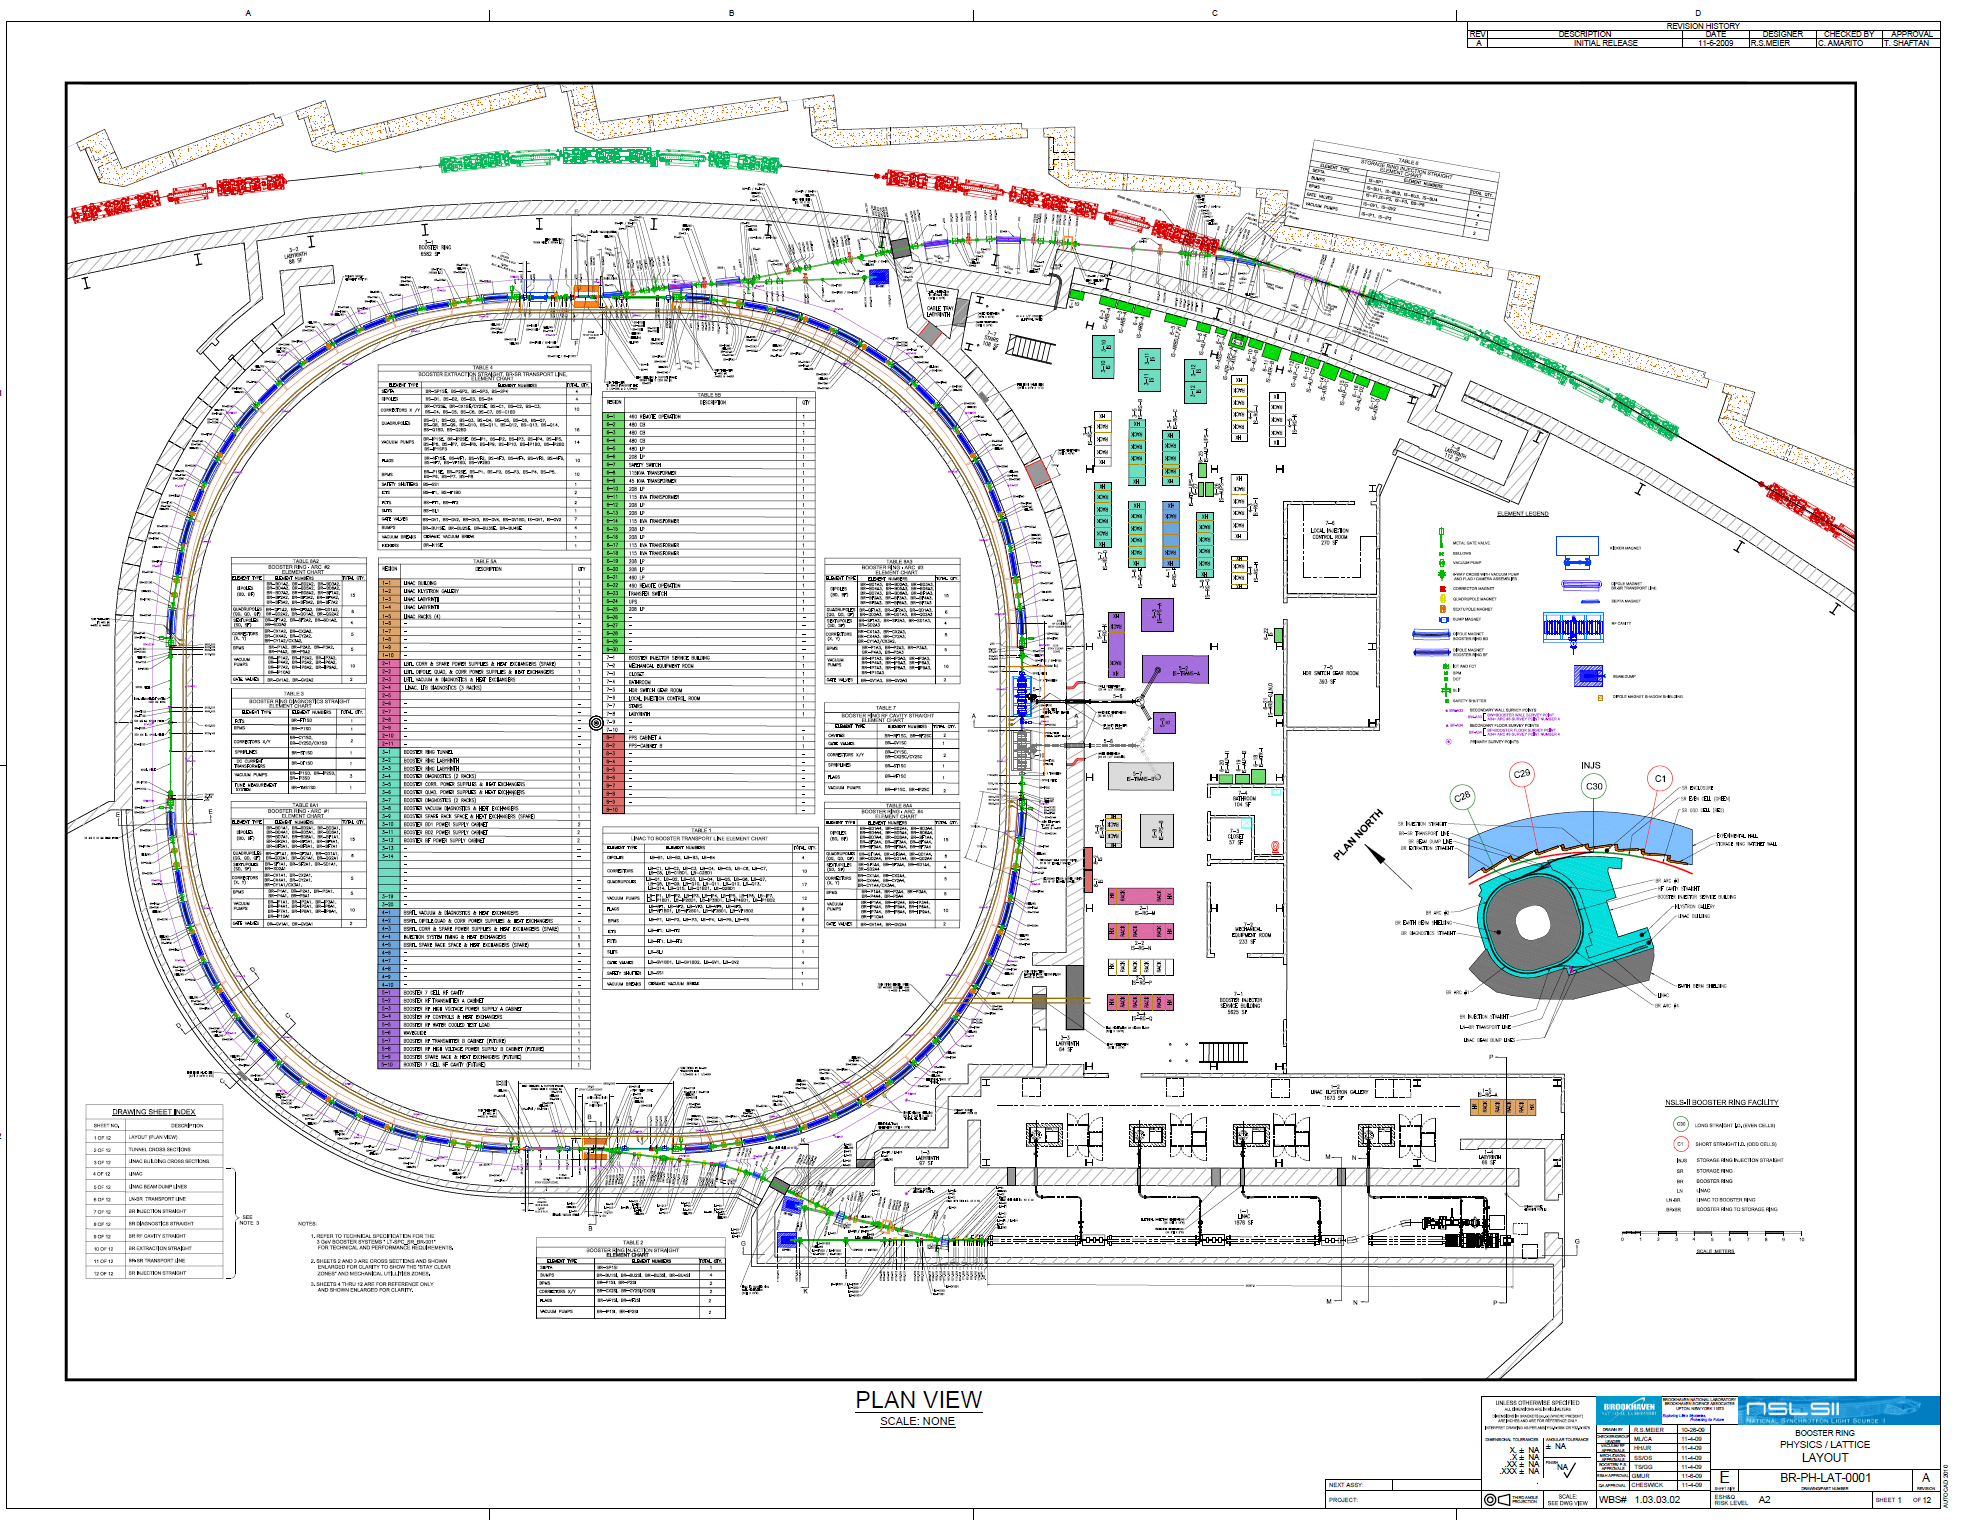
\includegraphics[width=16.7cm]{map.png}
\caption*{Şekil 6. NSLS-II Enjektörünün düzeni.}
	\end{figure}
	
NSLS-II depolama halkasının çevresi 792 m'dir. Elektronları halka ve düz bölümler boyunca yönlendiren ve yerleştirme cihazlarını kurmak için kullanılabilen mıknatısların düzenine depolama halkası örgüsü denir. NSLS-II depolama halkası örgüsü, yaklaşık 60 demet hattını barındıracak 30 mıknatıs dizisinden veya çift bükücü akromat (DBA) hücrelerinden oluşur. NSLS-II, 30 hücreli (15 süper periyot) çift bükücü akromat örgüsü, 6.6 m uzunluğunda 15 düşük beta düz bölümü ve 9,3 m uzunluğunda 15 yüksek beta düz bölümü olan 3 GeV depolama halkası sinkrotron ışınım kaynağıdır. Damping Wigglers için üç uzun düz bölüm kullanılır (1,85 T tepe alanı, 0,1 m periyot uzunluğu ve 7 m uzunluk), bu da yatay yayınımı 2,05 nm-rad'dan 1 nm-rad'a düşürmektedir [9]. Ayrıca,

\begin{itemize}
    \item Kızılötesinden, yumuşak x-ışınlarına kadar foton enerjilerini kapsayan geniş bant kaynakları sağlayan 31 bükücü mıknatıs bağlantı noktası. Bu portlardan herhangi biri, alternatif olarak, sert x-ışını aralığını kapsayan üç kutuplu bir wiggler portu ile değiştirilebilir.
    
    \item Çok uzak kızılötesi ışık için büyük boşluk dipolleri üzerinde 4 bükücü mıknatıs bağlantı noktası.
    
    \item Ek demet hattı kapasitesi için tek bir düz bölüme birden fazla cihaz eklenebilir.
\end{itemize}


\newpage

	\begin{figure}[h]
 \centering
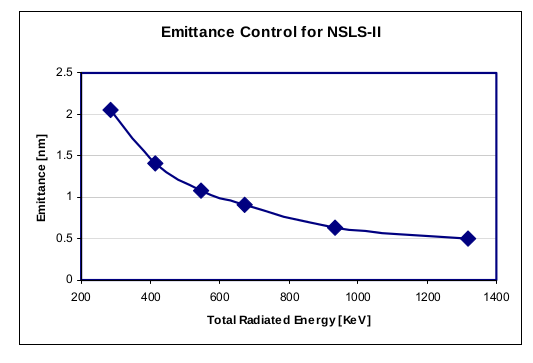
\includegraphics[width=13cm]{emittence.png}
\caption*{
\centering
Şekil 7. NSLS-II için 0, 1, 2, 3, 5 ve 8 DW (her biri 7 m) olarak yayınım azaltımı 1,8 T tepe alanında kurulur ve çalıştırılır [8].}
	\end{figure}
	
	\  
	
	\ 
	
		\begin{figure}[h]
 \centering
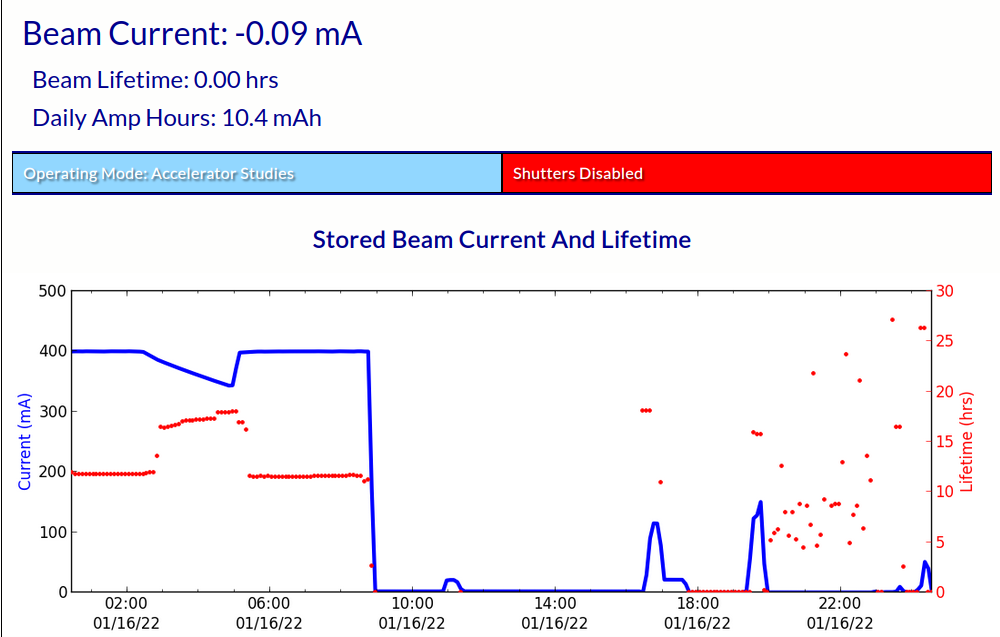
\includegraphics[width=13cm]{status.png}
\caption*{Şekil 8. NSLS II İşlem durumu [11].}
	\end{figure} 
	
	
	\newpage

	
	\begin{figure}[h!]
 \centering
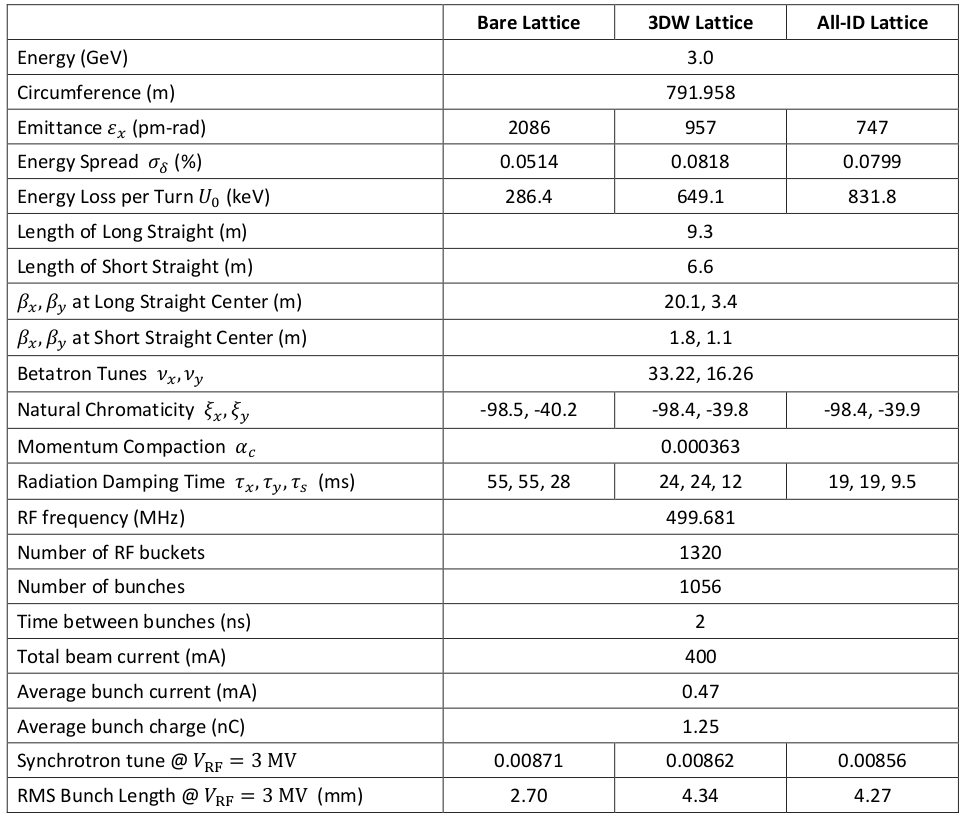
\includegraphics[width=15cm]{nsls parameter.png}
\caption*{Şekil 9. NSLS-II hızlandırıcı parametreleri [12].}
	\end{figure}
	
		\begin{figure}[h!]
 \centering
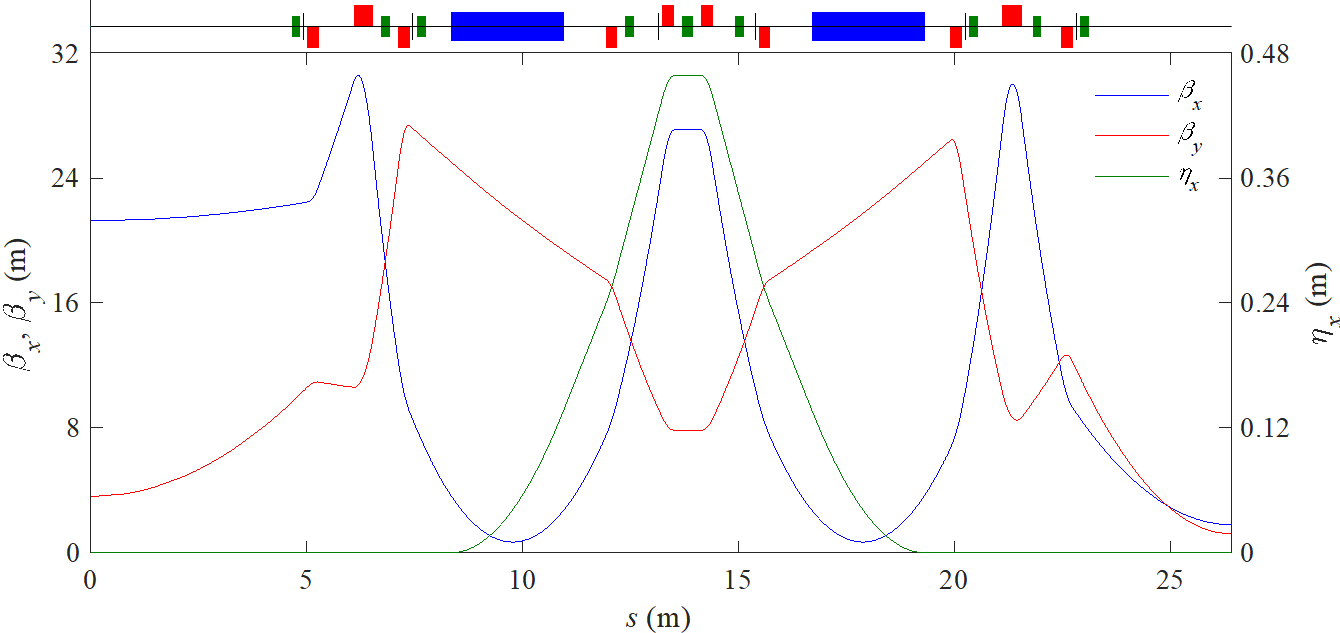
\includegraphics[width=12cm]{latticefunction.png}
\caption*{Şekil 10. NSLS-II Örgü fonksiyonları [12].}
	\end{figure}
	
	
	\newpage
\section{Enstrümanlar}	

Şu anda NSLS-II, yüksek verimli robot güdümlü numune işleme, yüksek uzaysal çözünürlüklü görüntüleme ve yüksek enerji çözünürlüğü dahil olmak üzere benzersiz, son teknoloji araştırma araçları sunan 28 demet hattı çalışmaktadır. NSLS-II'deki tüm demet hatları, sundukları araştırma yeteneklerine ve personel uzmanlığına dayalı olarak beş foton bilimi programına sahiptir [3].

Mevcut demet hatları portföyünün ötesinde, NSLS-II, halihazırda geliştirilmekte olan dört yeni demet hattı ile ek 30 demet hattı kapasitesine sahiptir. Tüm araştırma araçlarının her zaman son teknoloji olmasını sağlamak için, dedektörler, x-ışını optiği, hassas mühendislik ve konumlandırmanın yanı sıra teorik simülasyonlar üzerinde çalışan uzmanlardan oluşan bir ekibe sahiptir [3].

\subsection{Bilim Programları}

Brookhaven Ulusal Laboratuvarı'ndaki Ulusal Sinkrotron Işınım Kaynağı II (NSLS-II), dünyadaki en yeni, en gelişmiş üçüncü nesil sinkrotron radyasyon tesislerinden biridir. ABD Enerji Bakanlığı Bilim Kullanıcı Tesisi Ofisi olarak NSLS-II, dünya standartlarında yetenekler sağlayarak büyüyen kullanıcı topluluğunun nano ölçekli çözünürlük ve mükemmel hassasiyetle materyalleri incelemesini sağlar. NSLS-II'nin ışın hatları ve deney istasyonları, yüksek verimli robot güdümlü numune işleme, x-ışını saçılımı, benzeri görülmemiş enerji çözünürlüğü x-ışını mikroskobu dahil benzersiz, son teknoloji araştırma araçlarına sahiptir. Demet hatları, sundukları araştırma tekniklerine dayalı olarak beş bilimsel program halinde düzenlenmiştir [13].

\begin{itemize}
    \item Kompleks Saçılma (Complex Scattering)
    
    \item Görüntüleme ve Mikroskopi (Imaging and Microscopy)
    
    \item Yapısal Biyoloji (Structural Biology)
    
    \item Sert X-ışını Saçılımı ve Spektroskopisi (Hard X-ray Scattering \& Spectroscopy) 
    
    \item Yumuşak X-ışını Saçılımı ve Spektroskopisi (Soft X-ray Scattering \& Spectroscopy) 
\end{itemize}


		\begin{figure}[h!]
 \centering
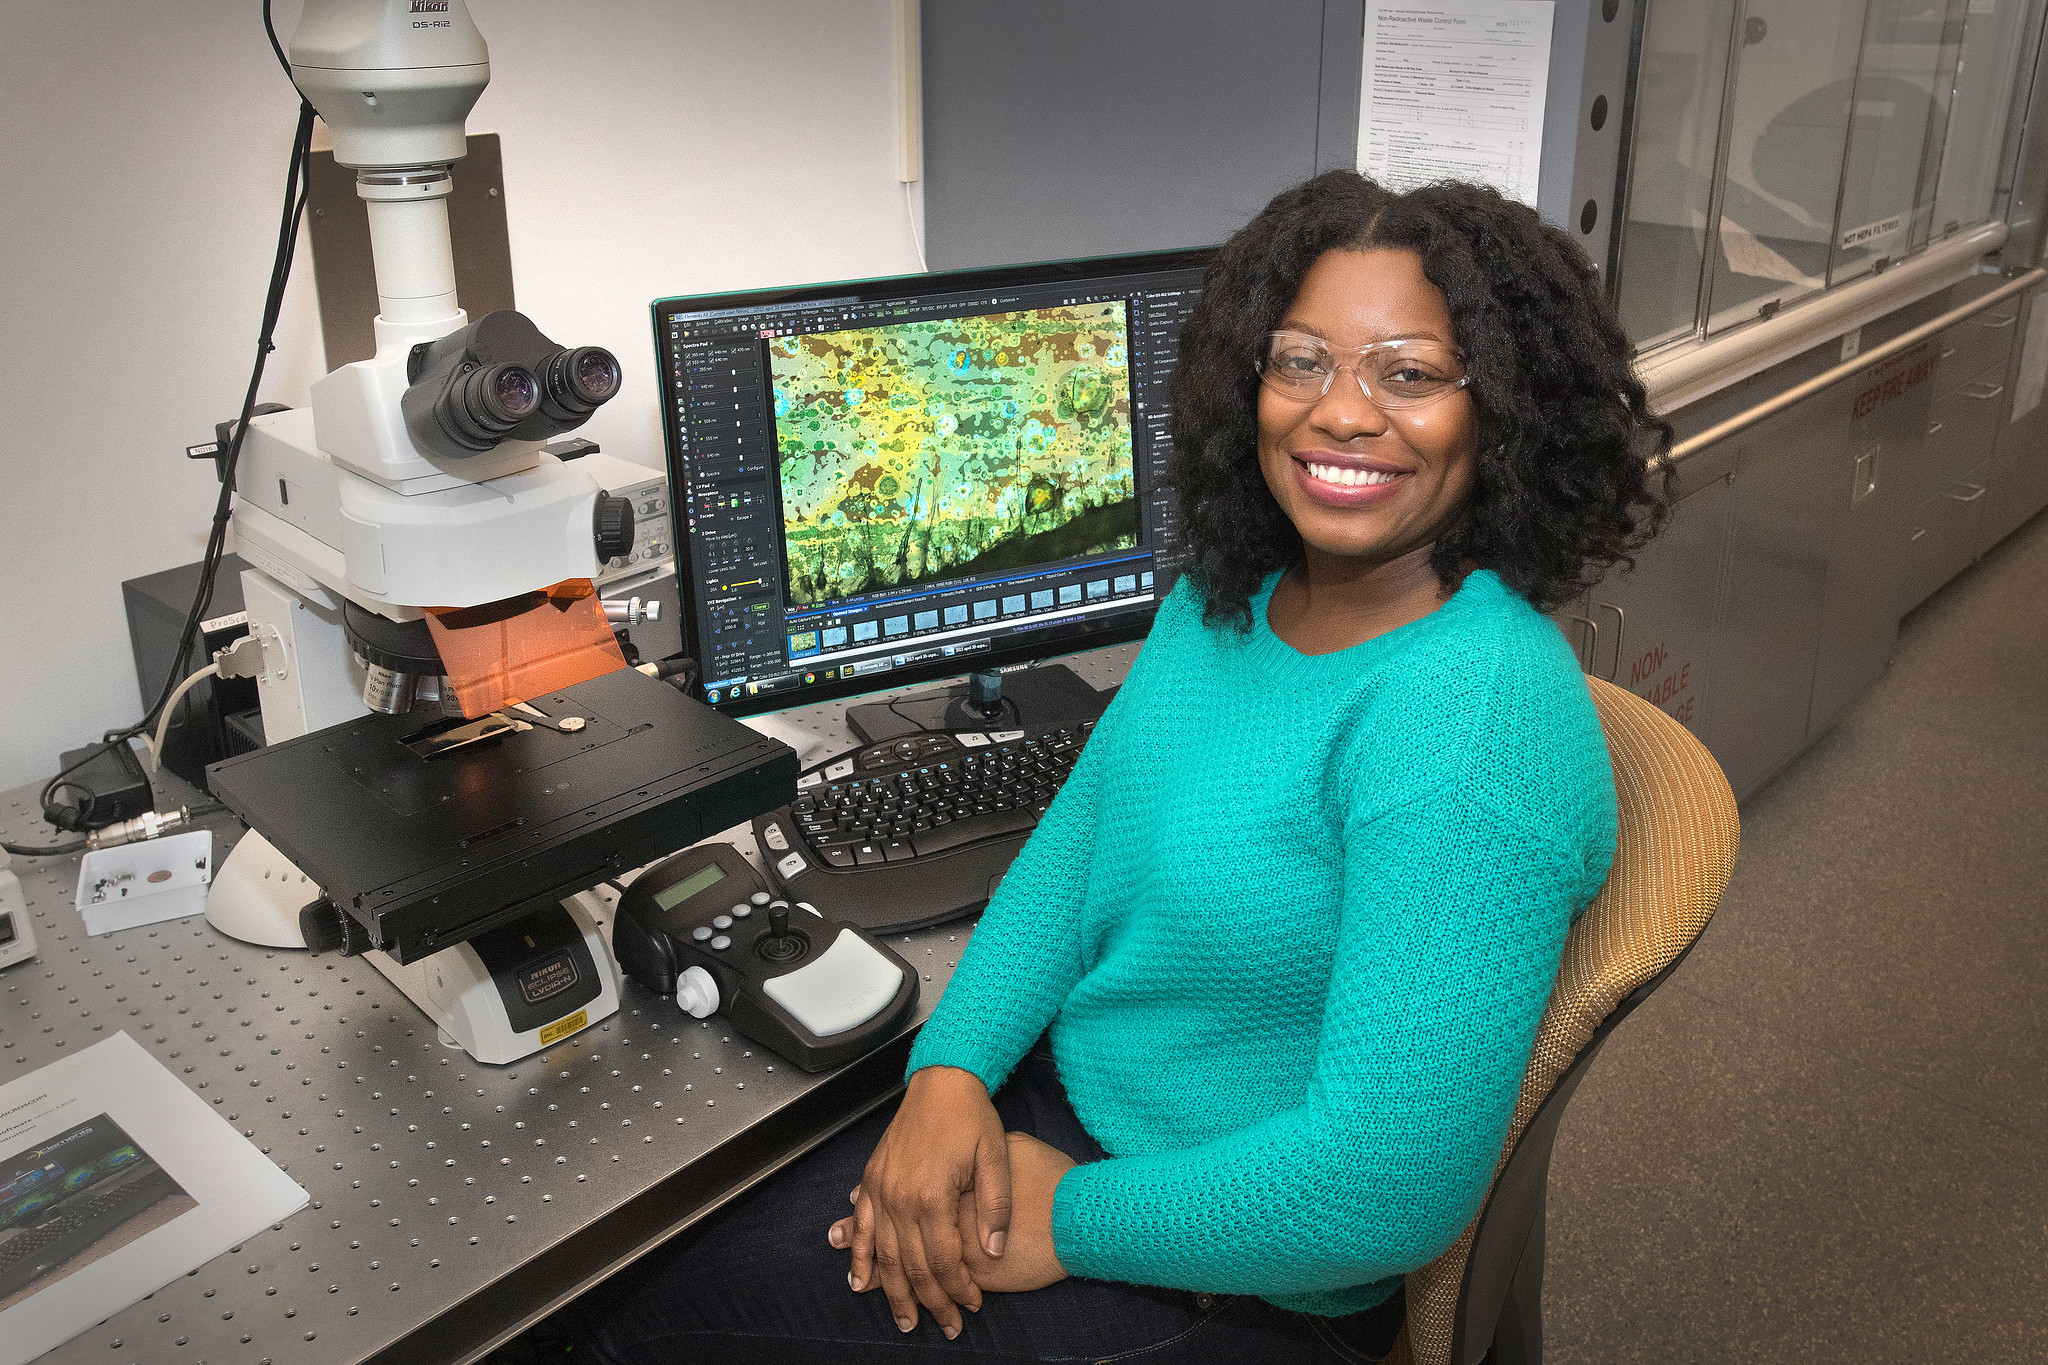
\includegraphics[width=13cm]{33696668366_c810eac721_k.jpg}
\caption*{Şekil 11. NSLS-II'de Biyoyakıt araştırması [14].}
	\end{figure}
	


\newpage

		\begin{figure}[h!]
 \centering
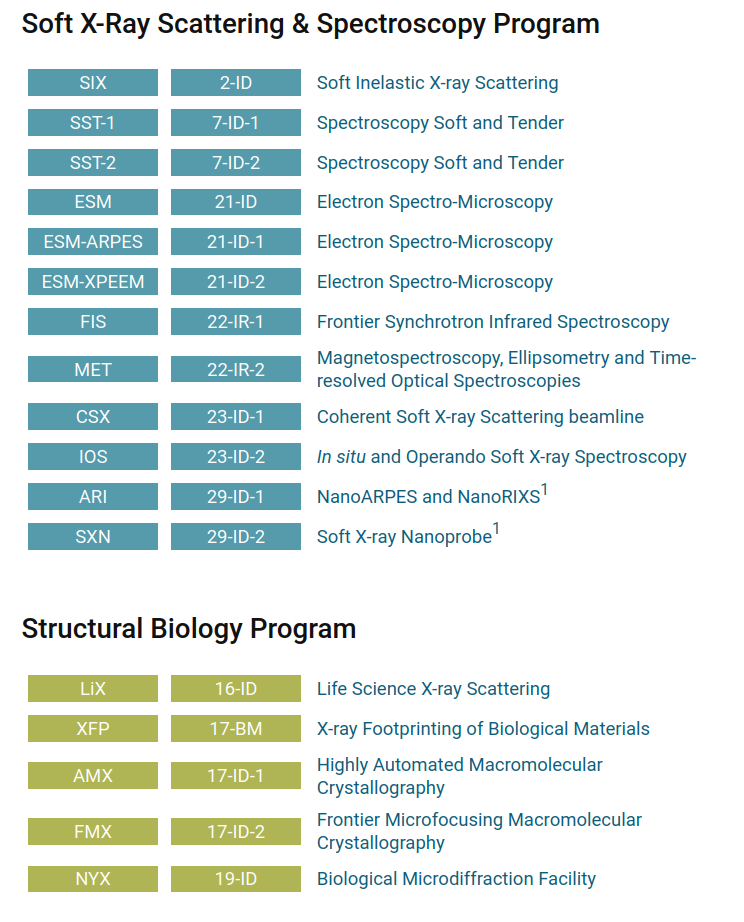
\includegraphics[width=12cm]{program1.png}
\caption*{Şekil 12. Demet hatları ve kullanıldığı bilim programı [12].}
	\end{figure}
	
\newpage

			\begin{figure}[h!]
 \centering
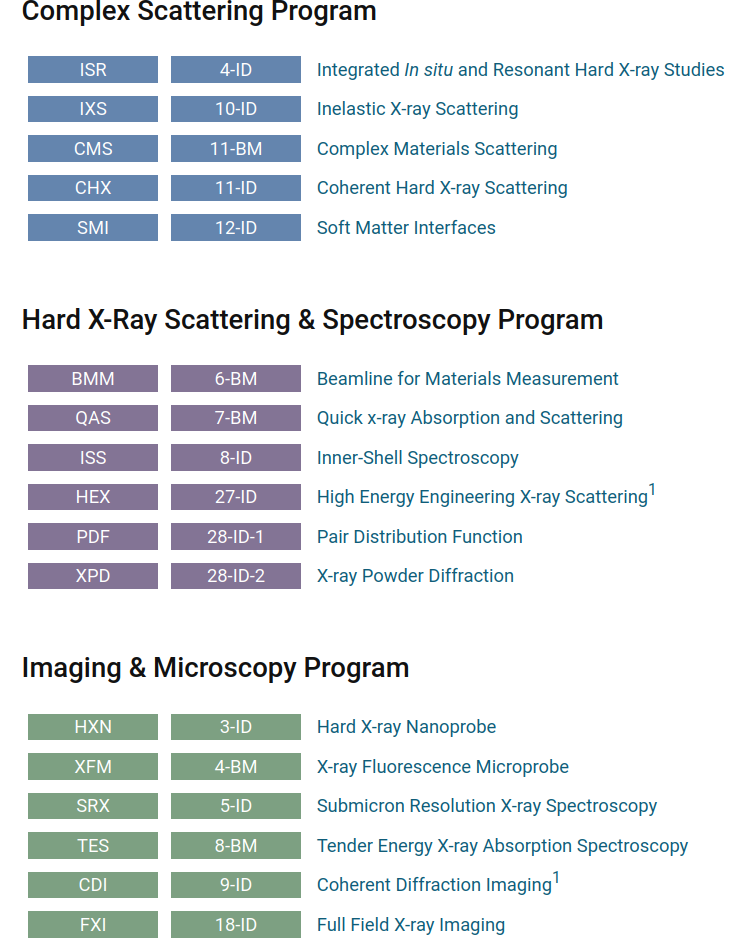
\includegraphics[width=12cm]{program 2.png}
\caption*{Şekil 13. Demet hatları ve kullanıldığı bilim programı [12].}
	\end{figure}


\section{Gelecek Planlar}
NSLS-II Ekibinin önümüzdeki 5 yıllık stratejileri:

\begin{itemize}
    \item Güvenilir kullanıcı operasyonlarında 500 mA ve 8 pm-rad dikey yayınımlı olgun hızlandırıcı performansı sağlamak
    \item Mevcut demet hatlarını yeniden sermayelendirmek ve COVID sonrası dönemde yeni erişim modaliteleriyle rekabet etmelerini sağlamak
    \item Veri depolama ve analizini geliştirmek
    \item HEX demet hattını ve NEXT-II projesini tamamlamak
    \item Tesisin konumunu gelecek on yılda yükseltmek
\end{itemize}



\newpage
\section{Kaynakça}

	\begin{thebibliography}{99}
	\bibitem{mano} (Dijital Görsel) \textit{National Synchrotron Light Source II (NSLS-II)}. Erişim adresi: \url{https://science.osti.gov/bes/suf/User-Facilities/X-Ray-Light-Sources/NSLS-II}. Erişim tarihi: 03.01.2022.
	
	\bibitem{mano} National Synchrotron Light Source II. InWikipedia, Özgür Ansiklopedi. \url{https://en.wikipedia.org/wiki/National_Synchrotron_Light_Source_II}. Erişim tarihi: 03.01.2022.  
	
	\bibitem{mano} About NSLS-II (n.d.). Erişim adresi: \url{https://www.bnl.gov/nsls2/about-nsls-ii.php} Erişim tarihi: 03.01.2022.
	
	\bibitem{mano} Accelerator Division (n.d.). Erişim adresi: \url{https://www.bnl.gov/nsls2/accelerator/} Erişim tarihi: 03.01.2022.
	
	\bibitem{mano} National Synchrotron Light Source II (2021). \textit{2022 NSLS-II Strategic Plan}. Erişim adresi: \url{https://www.bnl.gov/nsls2/docs/pdf/nsls2-strategic-plan.pdf} Erişim tarihi: 03.01.2022.
	
	\bibitem{mano} (Dijital Görsel) \textit{NSLS-II Beamline Map} Erişim Adresi: \url{https://www.bnl.gov/nsls2/beamlines/map.php}. Erişim tarihi: 07.01.2022.
	
	 \bibitem{mano} Accelerator Division (n.d.). Erişim adresi: \url{https://www.bnl.gov/nsls2/accelerator/machine.php} Erişim tarihi: 16.01.2022.
	 
	  \bibitem{mano} Dierker, S. (2007). \textit{National Synchrotron Light Source II
Preliminary Design Report}. Erişim adresi: \url{https://www.bnl.gov/isd/documents/75003.pdf} Erişim tarihi: 16.01.2022.
	
	
	\bibitem{mano} Wang, G. et al. (2016). \textit{NSLS-II commissioning and operation.} AIP Conference Proceedings 1741, 020007. doi:10.1063/1.4952786.
	
	\bibitem{mano} Gurov S. et al. (2014). \textit{The NSLS-II Booster Commissioning.}  Proc. 5th Int. Particle Accelerator Conf. (IPAC'14), Dresden, Germany, 295-297. doi:10.18429/JACoW-IPAC2014-MOPRO088.
	
	\bibitem{mano} (Dijital Görsel) \textit{NSLS II Operations Status} Erişim Adresi: \url{https://status.nsls2.bnl.gov/}. Erişim tarihi: 16.01.2022.
	
	 \bibitem{mano} NSLS-II Accelerator Parameters (n.d.). Erişim adresi: \url{https://www.bnl.gov/nsls2/accelerator/docs/accelerator-parameters.pdf} Erişim tarihi: 16.01.2022.

   \bibitem{mano} Science Programs (n.d.). Erişim adresi: \url{https://www.bnl.gov/nsls2/programs/} Erişim tarihi: 16.01.2022.
   
   \bibitem{mano} (Dijital Görsel) \textit{Biofuel Research at NSLS-II} Erişim Adresi: \url{https://www.flickr.com/photos/brookhavenlab/33696668366/in/album-72157615585907461/}.
   Erişim tarihi: 16.01.2022.
   

	\end{thebibliography}
	


\end{document}
